\section{Framebuffer 與輸出}
\label{sec:framebuffer}

\subsection{Color Buffer 與畫面還原}

ColorBuffer 以 RGBA 儲存 framebuffer，透過 \lstinline|glReadPixels()| 擷取畫面，再以 \lstinline|glDrawPixels()| 還原。Window 分別記錄「內容需要重畫」與「畫面需要重新擷取」兩種狀態：Scene 或版面改變時先重畫 Element tree，畫面穩定後再更新 cache；若只是視窗重新曝光，則直接還原像素。圖~\ref{fig:color-buffer-flow} 顯示狀態轉換，座標、pixel row 與 OpenGL state 的處理詳見附錄~\ref{app:framebuffer-details}。

\begin{figure}[tbp]
    \centering
    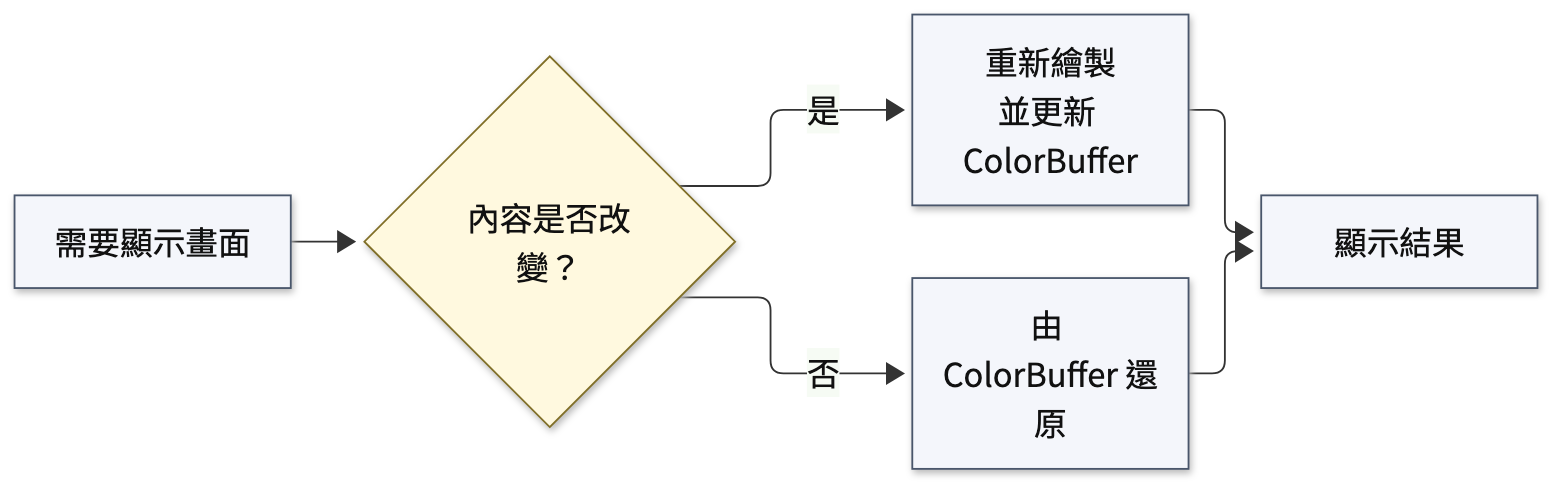
\includegraphics[width=.94\textwidth]{docs/figures/ch06_color-buffer-flow.png}
    \caption{ColorBuffer 快取與畫面還原流程}
    \label{fig:color-buffer-flow}
\end{figure}

\subsection{圖片輸出}

輸出圖片時，程式建立與 Canvas 同尺寸的 GraphicsRenderWindow，關閉 Grid，並重用 Canvas Renderer 繪製 Scene。完成後將 framebuffer 由下到上的 RGBA rows 轉為由上到下的 RGB rows，再寫成 PPM P6；因此輸出不包含主視窗的 Grid 與狀態列。PNG 與 JPEG 目前尚未實作。

圖~\ref{fig:ppm-result} 的實際輸出尺寸為 $800\times578$。自由曲線與中文字方向正確，且沒有 Grid 與狀態列，可確認圖片輸出只重新繪製 Scene 內容。
